\chapter{Triển khai hệ thống}\label{chap3}
Ở Chương~\nameref{chap2} khóa luận đã đề cập đến một số công nghệ được sử dụng trong quá trình thiết kế như Kubernetes, RabbitMQ, MongoDB, v.v.
Mỗi công nghệ được lựa chọn và sử dụng trong quá trình phát triển hệ thống đều đóng một vai trò quan trọng giúp đảm bảo luồng nghiệp vụ phía người dùng diễn ra một cách mượt mà và toàn vẹn.
Chương này sẽ đi chi tiết hơn vào diễn giải cách các công nghệ này tương tác, hoạt động với nhau, lợi ích của từng công nghệ cụ thể.
Tiếp sau đó, Mục~\nameref{sec:deploy-environment} sẽ trình bày cách triển khai hệ thống quản lý quán ăn lên môi trường đám mây của Google Cloud quá trình cài đặt HPA giúp hệ thống tự động mở rộng (autoscale) khi có lưu lượng truy cập lớn.
\section{Công nghệ sử dụng} \label{sec:tehcnologies-used}
\subsection{Kubernetes (K8s)}
Đối với mô hình quản lý quán ăn tập trung, việc đảm bảo khả năng chịu lỗi và tính sẵn sàng cao khi các quán ăn sử dụng hệ thống là điều thiết yếu.
Điều này đặc biệt đúng trong giờ cao điểm khi các nhà hàng, quán ăn đón một lượng lớn khách hàng đến quán.
Từ đó khóa luận này đưa ra phương án thiết kế hệ thống đi theo mô hình hệ thống phân tán (distributed system) với kiến trúc vi dịch vụ sử dụng K8s nhằm đạt được những yêu cầu đề ra và hơn thế nữa.

Khi sử dụng mô hình phân tán, hệ thống sẽ tránh được việc có một điểm lỗi duy nhất (single point of failure), khi một dịch vụ ngừng hoạt động, chỉ có riêng phần chức năng đó của hệ thống dừng phản hồi trong thời gian quản trị viên sửa chữa dịch vụ lỗi.
Về phía khách hàng cũng như là quán ăn, trải nghiệm sử dụng của họ trên toàn bộ hệ thống sẽ dường như không thay đổi và đây là một ưu điểm lớn trong mô hình phân tán.
Ngoài ra các hệ thống/dịch vụ độc lập với nhau thuộc hệ phân tán còn mang lại lợi ích cho khả năng mở rộng, phát triển nhờ sự tách biệt về mặt công nghệ.
Các đội ngũ kỹ thuật hoàn toàn có thể phát triển hệ thống/dịch vụ của đội mà không gây ảnh hưởng đến các đội khác.
Một ví dụ cho lợi ích này đó là dịch vụ thông báo.
Như đã nói đề cập ở Mục~\nameref{sec:system-architecture}, dịch vụ thông báo sẽ đóng vai trò giao tiếp với mọi dịch vụ khác trong hệ thống mỗi khi có một đơn đặt bàn mới, một lời gọi món mới, v.v.
Khi vào giờ cao điểm, dịch vụ thông báo sẽ cần phải điều phối lượng thông tin của mọi dịch vụ khác gửi đến và có thể gây ra hiện tượng tắc nghẽn cho toàn bộ hệ thống nếu không mở rộng dịch vụ này.
Nếu hệ thống được triển khai theo mô hình kiến trúc một khối (monolithic), việc nâng cấp chỉ riêng tính năng thông báo sẽ đồng nghĩa với việc phải nâng cấp cho toàn bộ máy chủ của toàn bộ tất cả các dịch vụ khác.
Quá trình này không những khó khăn và tốn kém hơn mà còn khiến cho toàn bộ hệ thống chịu ảnh hưởng từ một dịch vụ.
Bằng cách triển khai dịch vụ thông báo trên một máy chủ độc lập, ta sẽ loại bỏ được những phiền toái ban đầu liên quan đến phát triển, nâng cấp cũng như là bảo trì, sửa chữa.

Một trong những kiến trúc phổ biến nhất của mô hình hệ thống phân tán đó là kiến trúc vi dịch vụ.
Các lợi ích chính của K8s có thể kể đến như là tự động hóa quá trình triển khai, mở rộng và quản lý các ứng dụng đóng gói (containerized).
Các ứng dụng đóng gói trong ngữ cảnh này là từng dịch vụ riêng lẻ đảm nhiệm cho từng chức năng chính trong hệ thống kiến trúc vi dịch vụ.
Trong quá trình phát triển phần mềm, mã nguồn luôn thay đổi và cập nhật liên tục để đáp ứng nhu cầu mới và sửa lỗi.
Việc triển khai thủ công các phiên bản mới có thể tốn thời gian và dễ xảy ra sai sót.
Vì vậy, việc sử dụng quy trình tự động triển khai của Kubernetes (K8s) là một giải pháp hợp lý.

Trong Kubernetes, việc triển khai ứng dụng được thực hiện trên một cụm (cluster), là một tập hợp các máy chủ (node) làm việc cùng nhau để cung cấp tài nguyên tính toán và lưu trữ~\footnote{https://kubernetes.io/docs/concepts/overview/components/}.
Đơn vị triển khai cơ bản của K8s là Pod, thông thường bên trong một Pod sẽ chỉ có duy nhất một container~\footnote{https://kubernetes.io/docs/reference/glossary/?fundamental=true\#term-container} chính nhưng Pod cũng được thiết kế cho nhiều container với liên kết chặt chẽ với nhau để thực hiện một chức năng cụ thể~\footnote{https://kubernetes.io/docs/reference/glossary/?fundamental=true\#term-pod}.
Các Pod được quản lý bởi Deployment, chịu trách nhiệm duy trì số lượng pod mong muốn và đảm bảo chúng luôn hoạt động.
Deployment được nhắc đến ở đây như một khái niệm trừu tượng, trên thực tế các Deployment không trực tiếp chạy trên bất kỳ máy chủ vật lý nào.
Chúng hoạt động như một bản thiết kế, mô tả trạng thái mong muốn của ứng dụng, bao gồm số lượng bản sao pod, phiên bản image và các cấu hình khác.

Các Pod được triển khai trên Worker Node, là các máy chủ vật lý trong cluster K8s.
Worker Node cung cấp tài nguyên tính toán và lưu trữ cho các Pod hoạt động.
Ngoài ra ta cũng có Master Node chịu trách nhiệm quản lý toàn bộ cluster, bao gồm việc lên lịch triển khai Pod, giám sát trạng thái Pod và đảm bảo tính sẵn sàng của hệ thống.
Trong một cụm hoàn toàn có thể có Master Node, tuy nhiên các Master Node sẽ tiến hành bầu cử để chọn ra một Master Node chính chịu trách nhiệm quản lý cụm và các Master Node còn lại sẽ đóng vai trò như bản sao của Node chính này.
Quá trình bầu cử này dựa vào thuật toán đồng thuận phân tán như Raft\footnote{Để giúp hiểu thêm về thuật toán đồng thuận phân tán, tham khảo trang http://thesecretlivesofdata.com/raft/} giúp đảm bảo tính công bằng, nhất quán và độ tin cậy của hệ thống.

Bên trong một cụm (cluster) K8s, các Pod sẽ giao tiếp với nhau bằng mạng nội bộ.
Như trên Hình~\ref{fig:k8s-cluster-network}, các Nodes tức các Worker Node và bên trong đó chứa các Pod/ứng dụng.
Các Pod này được quản lý bởi các Service nằm trong cụm K8s đó.
Mỗi Pod trong mạng sẽ được gán một địa chỉ IP (Internet Protocol) ảo và port (cổng) độc nhất trong mạng nội bộ bởi Service.
Service hoạt động như một bộ cân bằng tải nội bộ và giúp quản lý các Pod trong hệ thống.
Khi có yêu cầu đến Service, tùy thuộc vào cấu hình cân bằng tải, Master Node sẽ chỉ định một trong các Pod có trong Service xử lý yêu cầu đó.

Trước khi các yêu cầu từ bên ngoài đến được tới Service, K8s sử dụng Ingress để phân loại và điều hướng đến các Service phù hợp.
Ingress hoạt động như Controller (bộ điều khiển) ở tầng ứng dụng, tiếp nhận các yêu cầu từ ngoài Internet và dựa theo cấu hình được định nghĩa trước để chuyển hướng các yêu cầu đó tới các Service phù hợp.
Như trong Hình~\ref{fig:k8s-ingress} mô tả cách client gọi đến Ingress từ ngoài Internet sau đó được điều hướng về các Service dựa theo HTTP Header \tcode{Host} được truyền vào.
Bản thân Ingress cũng có thể đóng vai trò như một bộ cân bằng tải nhưng trong hệ thống khóa luận này phát triển sẽ không dùng tới nó.
Chi tiết về việc triển khai và các cấu hình của K8s trên hệ thống quản lý quán ăn sẽ được trình bày ở Mục~\nameref{sec:deploy-environment}.
\begin{figure}[H]
	\centering
	\includesvg[width=\textwidth]{images/hChip/K8s/kubernetes-cluster-network.svg}
	\caption{Các dải mạng khác nhau trong một cụm Kubernetes~\protect\footnotemark}
	\label{fig:k8s-cluster-network}
\end{figure}
\footnotetext{https://kubernetes.io/docs/concepts/cluster-administration/networking/\#kubernetes-ip-address-ranges}
\begin{figure}[H]
	\centering
	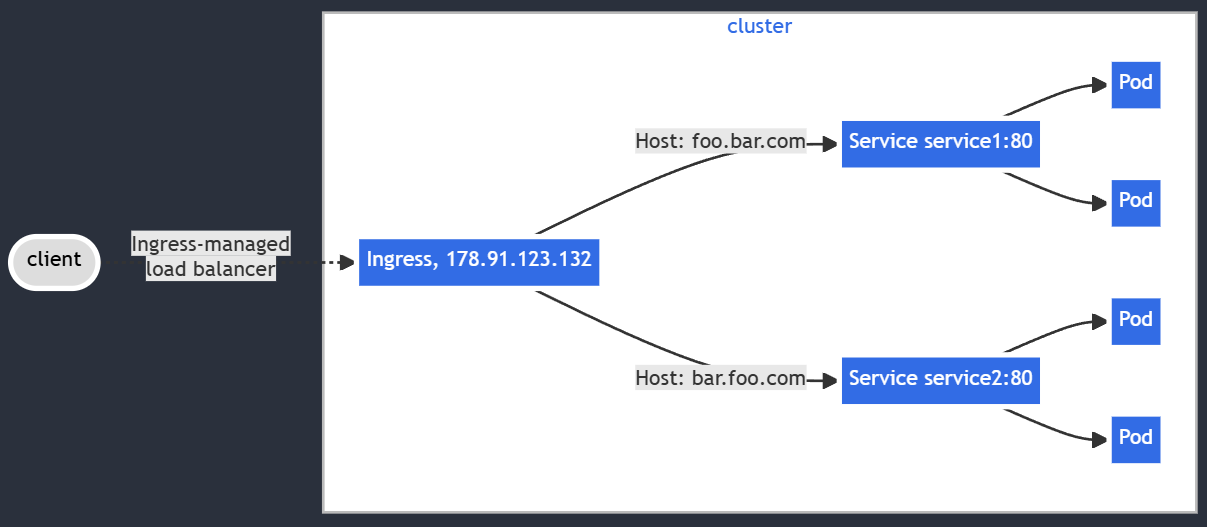
\includegraphics[width=\textwidth]{images/hChip/K8s/ingress-flow.png}
	\caption{Hình minh họa phân bố yêu cầu gọi đến các Service trong cụm ~\protect\footnotemark}
	\label{fig:k8s-ingress}
\end{figure}
\footnotetext{https://kubernetes.io/docs/concepts/services-networking/ingress/\#name-based-virtual-hosting}
\newpage
\subsection{RabbitMQ}
Đối với một hệ thống phân tán nói chung mà kiến trúc vi dịch vụ nói riêng, việc giao tiếp giữa các dịch vụ với nhau đóng vai trò then chốt.
Khác với các ứng dụng theo kiến trúc một khối (monolithic) truyền thống khi mà các thành phần giao tiếp với nhau thông qua các lời gọi hàm hoặc chia sẻ bộ nhớ, các ứng dụng theo kiến trúc vi dịch vụ giao tiếp với nhau qua hai hình thức chính:
\begin{itemize}
    \item Giao tiếp đồng bộ (Synchronous communication) là khi các dịch vụ gửi yêu cầu đến các dịch vụ đích và chờ phản hồi từ đó trước khi tiếp tục thực hiện tác vụ tiếp theo. Các giao thức phổ biến cho giao tiếp đồng bộ bao gồm RESTful API và gRPC.
    \item Giao tiếp bất đồng bộ (Asynchronous communication) khác với giao tiếp đồng bộ ở điểm dịch vụ gửi yêu cầu không cần chờ phản hồi ngay lập tức từ các dịch vụ đích.
    Điều này cho phép dịch vụ tiếp tục thực hiện các tác vụ khác trong khi chờ phản hồi.
    Giao tiếp không đồng bộ thường được thực hiện thông qua việc sử dụng hàng chờ tin nhắn (message queue).
\end{itemize}
Việc chọn ra một chuẩn giao tiếp phù hợp với ứng dụng trong quá trình thiết kế mang ý nghĩa quan trọng khi mà mỗi cách giao tiếp đều đi kèm những lợi ích và giới hạn riêng cho từng hệ thống cũng như là đội phát triển ứng dụng.
Hệ thống quản lý quán ăn yêu cầu khả năng xử lý các yêu cầu từ khách hàng một cách nhanh chóng, hiệu quả, từ đó khi thiết kế hệ thống, hàng đợi tin nhắn như một lựa chọn tốt nhất với những yêu cầu nghiệp vụ nói trên.
Điều này giúp các dịch vụ giảm sự phụ thuộc vào nhau khi chỉ cần biết địa chỉ của hàng đợi tin nhắn mà không cần biết địa chỉ của các dịch vụ khác trong cùng mạng.
Hàng đợi tin nhắn cũng giúp tránh thất thoát dữ liệu, một trường hợp có thể xảy ra là khi một dịch vụ không hoạt động, các tin nhắn vẫn được lưu trữ ở trong hàng đợi và sẽ được xử lý một khi dịch vụ đó trở lại hoạt động.

Các công nghệ hàng đợi tin nhắn (message broker) phổ biến trên thị trường hiện nay có thể kể đến bao gồm Kafka, RabbitMQ, Amazon Simple Queue Service, v.v.
Ở đây, RabbitMQ được lựa chọn nhờ sự đơn giản trong quá trình triển khai và cài đặt đơn giản hơn các dịch vụ khác.
Chi tiết về cách hàng đợi tin nhắn được sử dụng trong hệ thống quản lý quán ăn được đề cập ở Mục~\nameref{sec:system-architecture}.
\subsection{MongoDB}
Trong hệ thống quản lý nhà hàng phức tạp, việc lưu trữ và truy vấn dữ liệu hiệu quả là rất quan trọng.
Khác với các cơ sở dữ liệu truyền thống, MongoDB thuộc dạng cơ sở dữ liệu NoSQL, tức MongoDB có khả năng lưu trữ dữ liệu dạng tài liệu hay các dữ liệu phi cấu trúc một cách linh hoạt dưới dạng JSON. Điều này khiến cho cấu trúc bảng, dữ liệu có thể dễ dàng thích ứng với những thay đổi bất ngờ trong mô hình dữ liệu và yêu cầu nghiệp vụ.
Trong MongoDB, khái niệm khóa chính (primary key) và khóa ngoại (foreign key) không tồn tại theo cách hiểu truyền thống như trong các hệ quản trị cơ sở dữ liệu quan hệ (RDBMS). Tuy nhiên, MongoDB có những cơ chế riêng để đảm bảo tính toàn vẹn dữ liệu và tạo mối quan hệ giữa các bản ghi.
Đối với khóa chính, MongoDB tự động tạo một trường \tcode{\_id} cho mỗi tài liệu ngoại trừ những trường hợp người dùng chỉ định rõ.
Trường này có giá trị là một \tcode{ObejctId} duy nhất trên toàn bộ cơ sở dữ liệu.
Giá trị của \tcode{ObejctId} là một chuỗi \tcode{byte} dài 12 ký tự trong đó 4 \tcode{byte} mang giá trị là thời gian tạo \tcode{Id}, 5 \tcode{byte} là giá trị ngẫu nhiên được tạo ra dựa theo \tcode{Id} của tiến trình và của máy, cuối cùng là 3 \tcode{byte} được tạo với một bộ đếm tăng dần, bộ đếm này sẽ được khởi tạo với một giá trị ngẫu nhiên~\footnote{https://www.mongodb.com/docs/manual/reference/method/ObjectId/}.

Ngoài ra, MongoDB còn có một phiên bản dịch vụ đám mây gọi là MongoDB Atlas, mang lại nhiều lợi ích như khả năng mở rộng tài nguyên tự động, sao lưu và phục hồi dữ liệu, giám sát và cảnh báo, giúp giảm thiểu công việc quản trị và đảm bảo hệ thống luôn sẵn sàng phục vụ.

\begin{figure}[h]
	\centering
	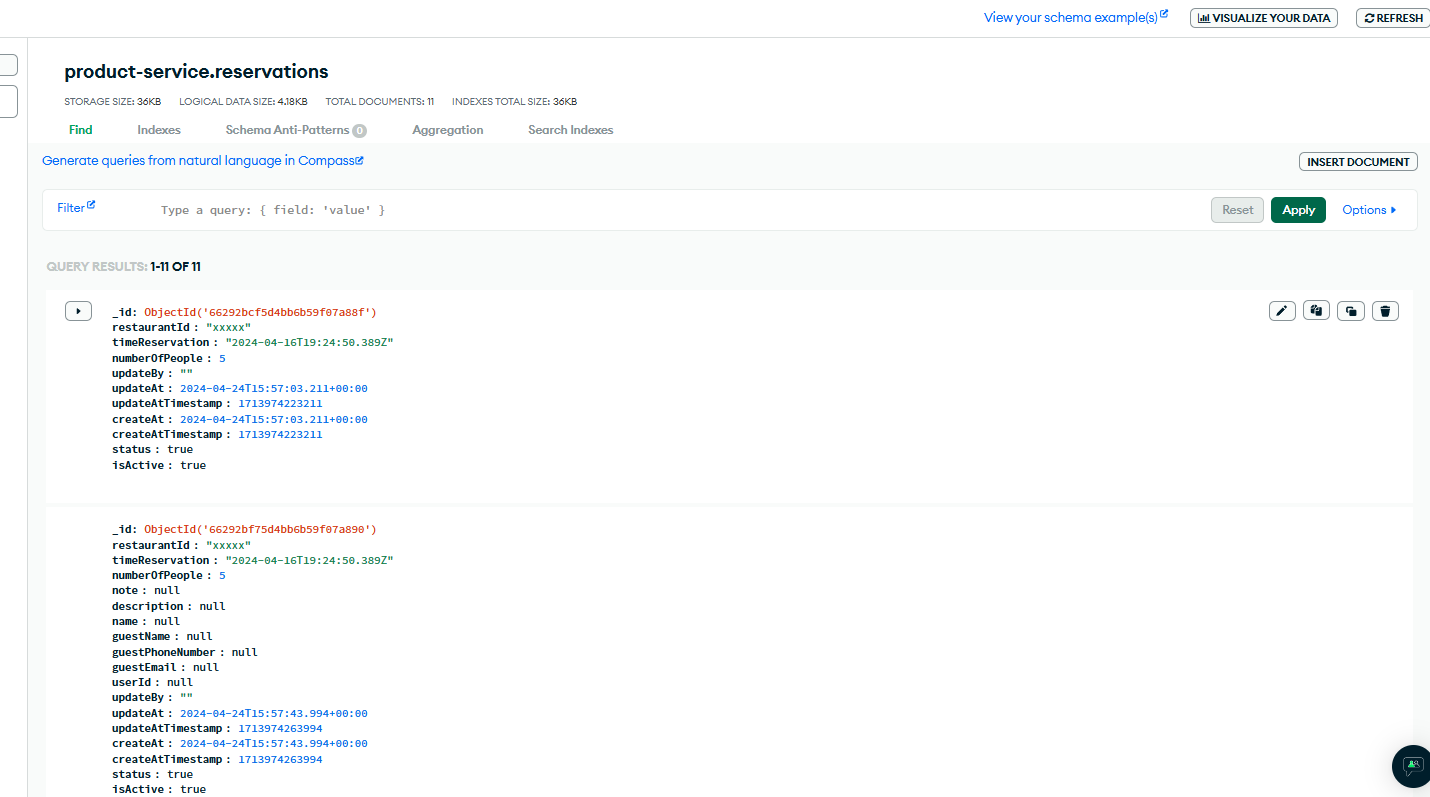
\includegraphics[width=\textwidth]{images/hChip/MongoDB/mongodb-preview.png}
	\caption{Giao diện người dùng của MongoDB Atlas}
	\label{fig:mongoDB-preview}
\end{figure}

Đối với một cơ sở dữ liệu thông thường, việc giám sát thông tin thường tập trung vào các loại như hiệu suất truy vấn, mức độ sử dụng tài nguyên, và trạng thái hoạt động.
Các chức năng này đều được MongoDB Atlas cung cấp trên nền tảng website gồm các chức năng như ghi nhật ký, các cảnh báo tùy chỉnh theo nhu cầu người dùng, giám sát tài nguyên hoạt động theo thời gian thực, v.v.
Từ đó khóa luận này quyết định sử dụng MongoDB cũng như là MongoDB Atlas làm cơ sở dữ liệu của hệ thống quản lý quán ăn.
Về chi tiết về mặt thiết kế cơ sở dữ liệu của hệ thống quản lý nhà hàng, quán ăn được đề cập ở Mục~\nameref{sec:database-design}.
\subsection{Kong}
Các hệ thống lớn hàng ngày sẽ phải tiếp nhận các lời gọi với tần suất rất lớn từ người dùng, đặc biệt là trong các giờ cao điểm trong ngày.
Không những thế, những hệ thống này còn có thể phải đối mặt với nguy cơ bị DDOS (Distributed Denial-of-Service), tức khi hệ thống bị ngợp bởi một lượng truy cập lớn có thể gây ra tê liệt hệ thống.
Cổng API (API Gateway) từ đây mang lại tác dụng như một điểm truy cập duy nhất cho ứng dụng, từ đó cấu hình chi tiết bên trong của nền tảng được ẩn dưới lớp API Gateway này.
Một trong những cổng API phổ biến đó là Kong Gateway.
Kong cung cấp các tiện ích khi sử dụng như chuyển đổi giao thức, đánh số, kiểm soát phiên bản API, giới hạn tốc độ truy cập và tích hợp các dịch vụ xác thực ở bên ngoài, v.v.

Khóa luận này thực hiện triển khai Kong Gateway trên một máy chủ thuộc GCP với Kong Manager.
Kiến trúc nền tảng của công gồm 3 thành phần bao gồm bộ định tuyển (router), dịch vụ (service), và máy chủ đích (upstream).
Khi nhận được yêu cầu từ ngoài vào, Kong Gateway sẽ khớp yêu cầu với Route phù hợp và chuyển tiếp yêu cầu đến Service tương ứng hoặc là tới các cân bằng tải đến cụm các Service trong Upstream.
Nhằm quản lý Kong dễn dàng và hiệu quả hơn, khóa luận sử dụng Kong Manager.
Kong Manager là bản thân Kong Gateway đã được trực quan hóa trên nền tảng web, điều này giúp người dùng dễ dàng tạo, chỉnh sửa và xóa các Route, Service và Upstream, phát triển, cấu hình các plugin nhằm mở rộng chức năng của Kong Gateway, giám sát lưu lượng truy cập API và hiệu suất của Kong.
\section{Quy trình triển khai}\label{sec:deploy-environment}
Trong bối cảnh phát triển các phần mềm hiện đại, khi mỗi dự án bao gồm nhiều đội ngũ phát triển phần mềm khác nhau với tần suất thay đổi mã nguồn ngày.
Nhằm lưu trữ, theo dõi các thay đổi một cách hiệu quả cũng như tăng cường hiệu quả phối hợp giữa các thành viên trong nhóm phát triển, các phần mềm quản lý mã nguồn (VCS - Version Control System) dần trở thành công cụ không thể thiếu trong giai đoạn phát triển cũng như là triển khai hệ thống.
Các VCS tiêu biểu có thể kể đến như là GitLab và GitHub, mặc dù cả hai nền tảng đều cung cấp đầy đủ các phương pháp quản lý mã nguồn hệ thống, cấu hình quyền người dùng linh hoạt và đều tích hợp các công cụ hỗ trợ kiểm thử hệ thống mạnh mẽ, GitLab nổi trội hơn GitHub về mặt tích hợp và triển khai liên tục (CI/CD) tốt hơn GitHub do cung cấp nhiều chức năng như bỏ qua các quy trình triển khai khi cần thiết, kết quả chạy đồng nhất và hiệu quả hơn, v.v. nên GitLab được lựa chọn là nền tảng quản lý mã nguồn cho hệ thống quản lý quán ăn.

Nền tảng quản lý quán ăn được chia làm tám kho lưu trữ mã nguồn (repository) bao gồm năm kho lưu trữ các mã nguồn thuộc về mặt logic của hệ thống, mỗi bộ mã nguồn tương dương với một vi dịch vụ và ba kho lưu trữ bao gồm trang giới thiệu (landing-page), trang quản lý nhà hàng (admin-page), và một trang mô phỏng phần đặt hàng của người dùng (customer-page).

Khi một thay đổi đối với mã nguồn được đẩy lên kho lưu trữ của GitLab, một quá trình kiểm tra và triển khai được cấu hình trước sẽ được chạy bởi GitLab Runner.
GitLab Runner là một ứng dụng chuyên biệt được phát triển bởi GitLab tích hợp với kho lưu trữ giúp chạy các câu lệnh cấu hình, kiểm thử và triển khai mã nguồn.
Ngoài lựa chọn sử dụng GitLab runner của riêng GitLab, việc tự triển khai riêng các GitLab Runner mang giúp khả năng tuỳ chỉnh cấu hình cụ thể của hạ tầng CI/CD, từ đó giúp tiết kiệm chi phí vận hành.

Có hai pha chính sẽ được thực hiện mỗi khi nhà phát triển phần mềm đẩy code lên kho mã nguồn của GitLab do GitLab Runner phụ trách đó là pha biên dịch mã nguồn và triển khai mã nguồn trên K8s và một pha phụ đó là cấu hình tệp \tcode{.env} cho mã nguồn trước đó giúp đẩy các biến môi trường giúp biên dịch mã nguồn.
Khi một thay đổi mới được đẩy lên GitLab, GitLab Runner sẽ tìm đọc tệp cấu hình \tcode{.gitlab-ci.yml} để xác nhận những chỉ dẫn cần được thực thi.

\begin{lstlisting}[style=yaml, caption={Đoạn mã cấu hình cài đặt biến môi trường cho GitLab Runner.}, label={cod:env-gitlab-ci/cd},  captionpos=b]
build_env:
  tags:
    - ${RUNNER_TAG}
  stage: build_env
  image: alpine/k8s:1.23.16
  script:
    - cat $PATH_DOCKER_BUILD_ENV_FILE > .env
  artifacts:
    paths:
      - .env
\end{lstlisting}

Đoạn mã~\ref{cod:env-gitlab-ci/cd} cho thấy cách đẩy tệp \tcode{.env} vào môi trường biên dịch.
Biến môi trường \tcode{\$PATH\_DOCKER\_BUILD\_ENV\_FILE} được sử dụng trong đoạn mã được cấu hình trong như một biến môi trường của dự án trên GitLab bên cạnh các biến môi trường khác được GitLab cung cấp sẵn khi chạy CI/CD.
Ở đây giá trị của biến là nội dung tệp \tcode{.env} là các biến hệ thống cần giúp cho hệ thống có thể biên dịch thành công bao gồm địa chỉ của kho lưu trữ ảnh và tệp trên Amazon S3, các biến trỏ đến đường dẫn các dịch vụ khác của hệ thống.

Sau khi mã nguồn trên kho lưu trữ của GitLab có tệp \tcode{env} cần thiết, GitLab Runner sẽ bắt đầu quá trình biên dịch mã nguồn hệ thống. Đoạn mã~\ref{cod:build-gitlab-ci/cd} sử dụng \tcode{kaniko} giúp chạy lệnh biên dịch mã nguồn sang ảnh Docker.
Kaniko~\footnote{https://github.com/GoogleContainerTools/kaniko} là một công cụ giúp xây dựng các ảnh Docker từ Dockerfile, có thể chạy bên trong một container hoặc một cụm K8s.
Kaniko giúp giải quyết hai vấn đề khi build Docker trong Docker (Docker-in-Docker)~\footnote{https://docs.gitlab.com/ee/ci/docker/using\_docker\_build.html\#use-docker-in-docker} đó là tránh việc phải chạy Docker ở quyền quản trị trong ảnh Docker, vốn là một điều phải có khi cần quyền truy cập vào Docker daemon của máy chủ, và giúp tối ưu quá trình chạy Docker-in-Docker (DinD) thông qua caching hiệu quả các lớp (layer) ảnh Docker~\footnote{https://cloud.google.com/blog/products/containers-kubernetes/introducing-kaniko-build-container-images-in-kubernetes-and-google-container-builder-even-without-root-access}.

\begin{lstlisting}[style=yaml, caption={Đoạn mã cấu hình quá trình biên dịch mã cho GitLab Runner.}, label={cod:build-gitlab-ci/cd},  captionpos=b]
build:
  stage: build
  tags:
    - ${RUNNER_TAG}
  image:
    name: gcr.io/kaniko-project/executor:debug
    entrypoint: [""]
  before_script:
    # - echo $IMAGE_REGISTRY_URL
    - echo $IMAGE_REGISTRY_USER
    # - echo $IMAGE_REGISTRY_PASS
    - echo "{\"auths\":{\"$IMAGE_REGISTRY_URL\":{\"auth\":\"$(printf "%s:%s" "$IMAGE_REGISTRY_USER" "$IMAGE_REGISTRY_PASS" | base64 | tr -d '\n')\"}}}" > /kaniko/.docker/config.json
    # - cat /kaniko/.docker/config.json
  script:
    - ls -la
    - cat .env
    - echo $IMAGE_NAME_BUILD
    - echo $IMAGE_NAME_BUILD_LATEST
    - /kaniko/executor
      --context "${CI_PROJECT_DIR}"
      --dockerfile "${CI_PROJECT_DIR}/Dockerfile"
      --cache=true
      --destination "$IMAGE_REGISTRY_URL/$IMAGE_NAME_BUILD_LATEST"
\end{lstlisting}

Trong Đoạn mã~\ref{cod:build-gitlab-ci/cd}, phần \tcode{before\_script} giúp người dùng đăng nhập vào một kho lưu trữ ảnh Docker (Docker Registry) giúp dễ dàng quản lý và triển khai trên K8s.
Sau đó GitLab Runner chạy phần \tcode{script} để biên dịch hệ thống dựa theo tệp \tcode{Dockerfile} được định nghĩa trước trong quá trình phát triển và kiểm thử hệ thống.

Cuối cùng pha triển khai (deploy) mã lên K8s của GCP, GitLab Runner được cấu hình chạy một tệp lệnh chương trình sử dụng kubectl, một công cụ giúp giao tiếp với các Master Node (Control Plane)~\footnote{https://kubernetes.io/docs/reference/kubectl/}.
Các cấu hình cho môi trường K8s nằm trong tệp \tcode{deployment-gke.yml} bao gồm các thành phần cài đặt cấu hình cho Ingress, Service và Deployment của hệ thống.
Đối với phần cấu hình cho Ingress và Service, K8s sẽ chỉ cần có số cổng mà ứng dụng mở ra ngoài và tên của kho mã nguồn, tuy nhiên ở phần cấu hình cho Deployment và autoscaling (tự động mở rộng), các trường thông tin sẽ ảnh hưởng nhiều đến hiệu năng của ứng dụng hơn như thông số của API kiểm tra tình trạng hoạt động, các thông số cấu hình phần cứng liên quan đến bộ nhớ và CPU cho mỗi Pod, và giới hạn số lượng pod tối đa khi hệ thống mở rộng cũng như là ngưỡng hệ thống quá tải cần mở rộng thêm.
\begin{lstlisting}[style=yaml, caption={Đoạn mã cấu hình cài đặt tự động mở rộng Kubernetes cho GitLab Runner.}, label={cod:k8s-gitlab-ci/cd},  captionpos=b, escapechar=|]
apiVersion: autoscaling/v2
kind: HorizontalPodAutoscaler
metadata:
  name: $CI_PROJECT_NAME
  namespace: $CI_PROJECT_ROOT_NAMESPACE
spec:
  scaleTargetRef:
    apiVersion: apps/v1
    kind: Deployment
    name: $CI_PROJECT_NAME
  minReplicas: 1
  maxReplicas: 5|\label{line:sp}|
  metrics:
    - resource:
        name: memory
        target:
          averageUtilization: 80
          type: Utilization
      type: Resource
    - resource:
        name: cpu
        target:
          averageUtilization: 50
          type: Utilization
      type: Resource
\end{lstlisting}
Nhằm phục vụ quá trình kiểm thử sản phẩm ở Chương~\nameref{chap4}, ngưỡng tự động mở rộng trong Đoạn mã~\ref{cod:k8s-gitlab-ci/cd} được đặt tại giới hạn sử dụng 80\% bộ nhớ và 50\% CPU.
Khi bất kỳ một Pod nào thuộc Deployment đạt tới ngưỡng, GKE sẽ tự động tạo thêm một Pod mới giúp giãn tải trên các Pod đang hoạt động, tới một giới hạn số lượng Pod tối đa là năm như được cấu hình tại Dòng~\ref{line:sp}, Đoạn mã~\ref{cod:k8s-gitlab-ci/cd}.
\section{Một số luồng chức năng chính}\label{sec:user-flow-examples}
Như đã nói ở Mục~\ref{sec:main-functions}, các luồng chính của nền tảng quản lý nhà hàng, quán ăn được mô tả sẽ bao gồm luồng đặt bàn của người dùng khách hàng tại quán ăn và luồng đặt đồ ăn thông qua việc quét mã QR từ phía người dùng.
Ở Chương này, ta sẽ đi sâu vào luồng di chuyển của người dùng cũng như là các lời gọi dữ liệu giữa các dịch vụ với nhau trong hệ thống.
\subsection{Luồng đặt bàn}\label{sec:reservation-sequence-flow}
Sơ đồ tuần tự ở Hình~\ref{fig:reservation-sequence-flow} mô tả cách người dùng tương tác với tính năng đặt hàng trên giao diện tại trang giới thiệu.
Sơ đồ tồn tại các tác nhân chính là người dùng/thực khách có nhu cầu đặt bàn, giao diện người dùng tương tác khi đặt bàn có thể từ trang giới thiệu nền tảng quản lý nhà hàng, quán ăn hoặc các trang riêng của nhà hàng có liên kết với hệ thống quản lý.
Tiếp theo đó là \tcode{product-service} tiếp nhận các lời gọi từ phía người dùng và xử lý chúng.
Hai tác nhân cuối gồm \tcode{admin-page} và nhân viên của cửa hàng phụ trách việc tiếp nhận, xác nhận lại yêu cầu đặt bàn của người dùng.

\begin{figure}[h]
	\centering
	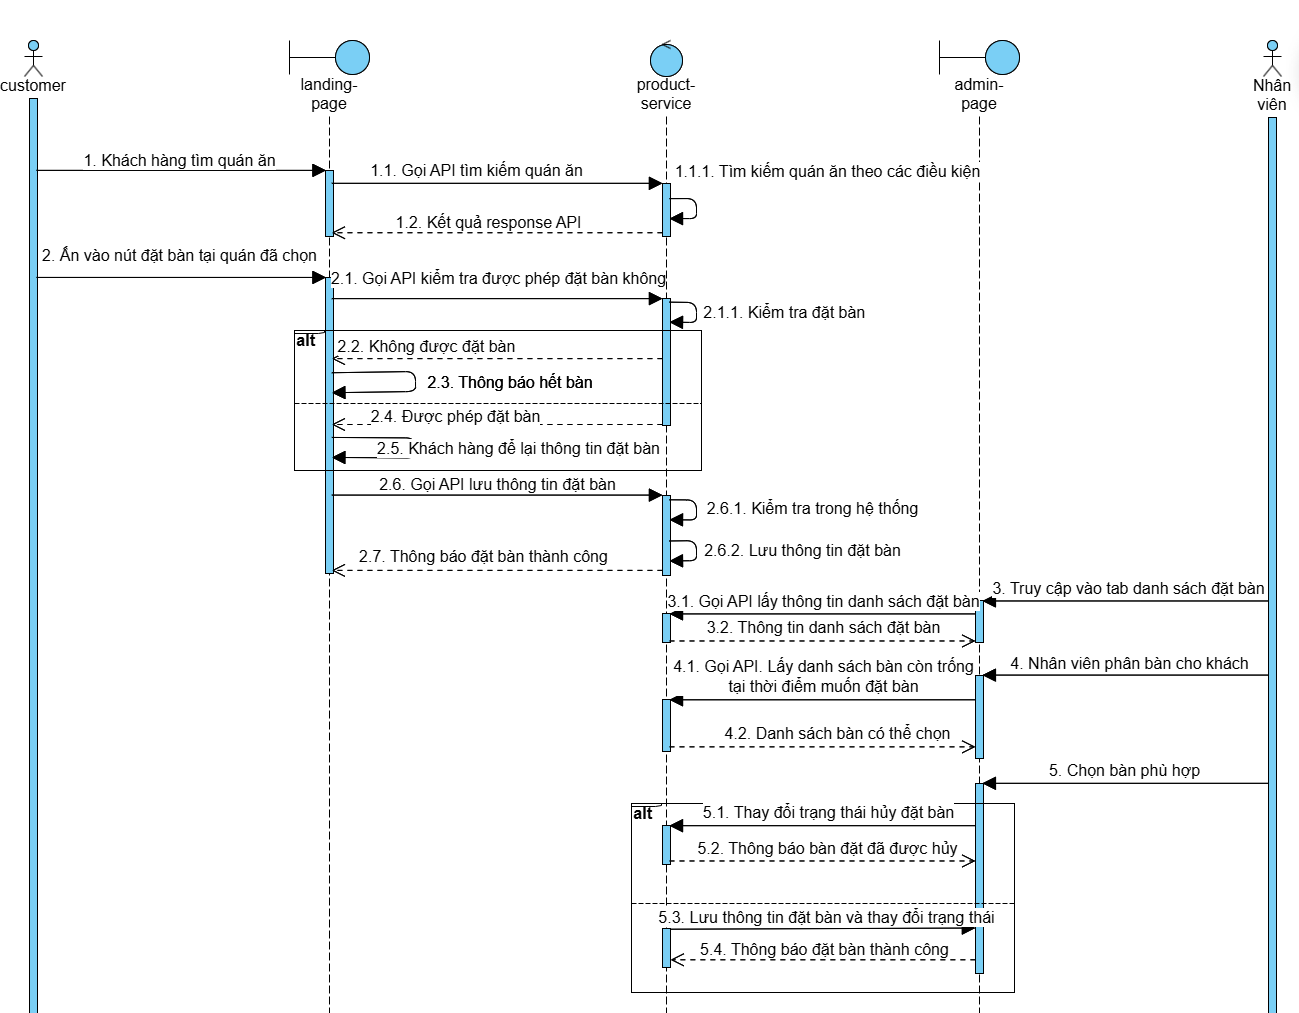
\includegraphics[width=\textwidth]{images/hChip/main-flow/reservation.png}
	\caption{Sơ đồ tuần tự mô tả luồng nghiệp vụ đặt bàn trực tuyến}
	\label{fig:reservation-sequence-flow}
\end{figure}

Luồng người dùng bắt đầu khi người dùng thực hiện tìm kiếm quán ăn trên trang giới thiệu của hệ thống hoặc của từng cửa hàng, khách hàng sẽ có lựa chọn đặt bàn tại quán ăn.
Sau khi khách hàng đã chọn xong bàn và điền các thông tin được yêu cầu, hệ thống sẽ kiểm tra tình trạng hiện tại của quán ăn và xác nhận lại với khách hàng tình trạng đặt bàn trên giao diện.
Một khi người dùng thực hiện đặt bàn thành công, thông tin sẽ được đẩy đến trung tâm thông báo và chuyển tiếp đến các dịch vụ khác, ở đây là trang quản lý nhà hàng. 
Nhân viên của quán ăn sẽ xác nhận yêu cầu đặt bàn của khách hàng và tiến hành phân bàn cho khách dựa trên số lượng, yêu cầu khi đặt bàn.
Nếu không thể chọn được bàn phù hợp cho yêu cầu của thực khách, nhân viên của quán ăn sẽ thay đổi trạng thái của phần đặt bàn thành đã hủy và ngược lại là thành công nếu có bàn.

Ở Hình~\ref{fig:reservation-sequence-flow} không có luồng thông báo cho người dùng về trạng thái đặt bàn do người đặt bàn có thể chưa đăng ký tham gia hệ thống, điều đó khiến cho việc thông báo cho người dùng trở nên khó khăn bởi hệ thống thông báo sẽ không biết thông tin của người dùng để hiển thị.
Nhân viên của quán sau khi thay đổi trạng thái của yêu cầu đặt bàn sẽ cần xác nhận, thông tin tới khách hàng theo dựa theo biểu mẫu mà khách cung cấp khi yêu cầu đặt bàn trên website.
\subsection{Luồng gọi món}\label{sec:order-sequence-flow}
Khi nhà hàng, quán ăn tham gia vào hệ thống quản lý sẽ được hỗ trợ tạo QR gán cho mỗi bàn thuộc nhà hàng giúp khách hàng có thể gọi món mà không cần tương tác với nhân viên của quán.
Hình~\ref{fig:order-sequence-flow} mô tả quá trình từ lúc người dùng sử dụng mã QR để đặt món và nhân viên, phục vụ của nhà hàng, quán ăn thay đổi trạng thái của đơn gọi món.
Các tác nhân trong sơ đồ bao gồm người dùng và nhân viên là hai tác nhân chính tương tác với hệ thống, trang \tcode{customer-page} giúp người dùng tương tác và thực hiện lời gọi đến hệ thống.
Các tác nhân đảm nhiệm việc xử lý bao gồm \tcode{order-service}, \tcode{product-service}, và \tcode{notification-service}.

\begin{figure}[h]
	\centering
	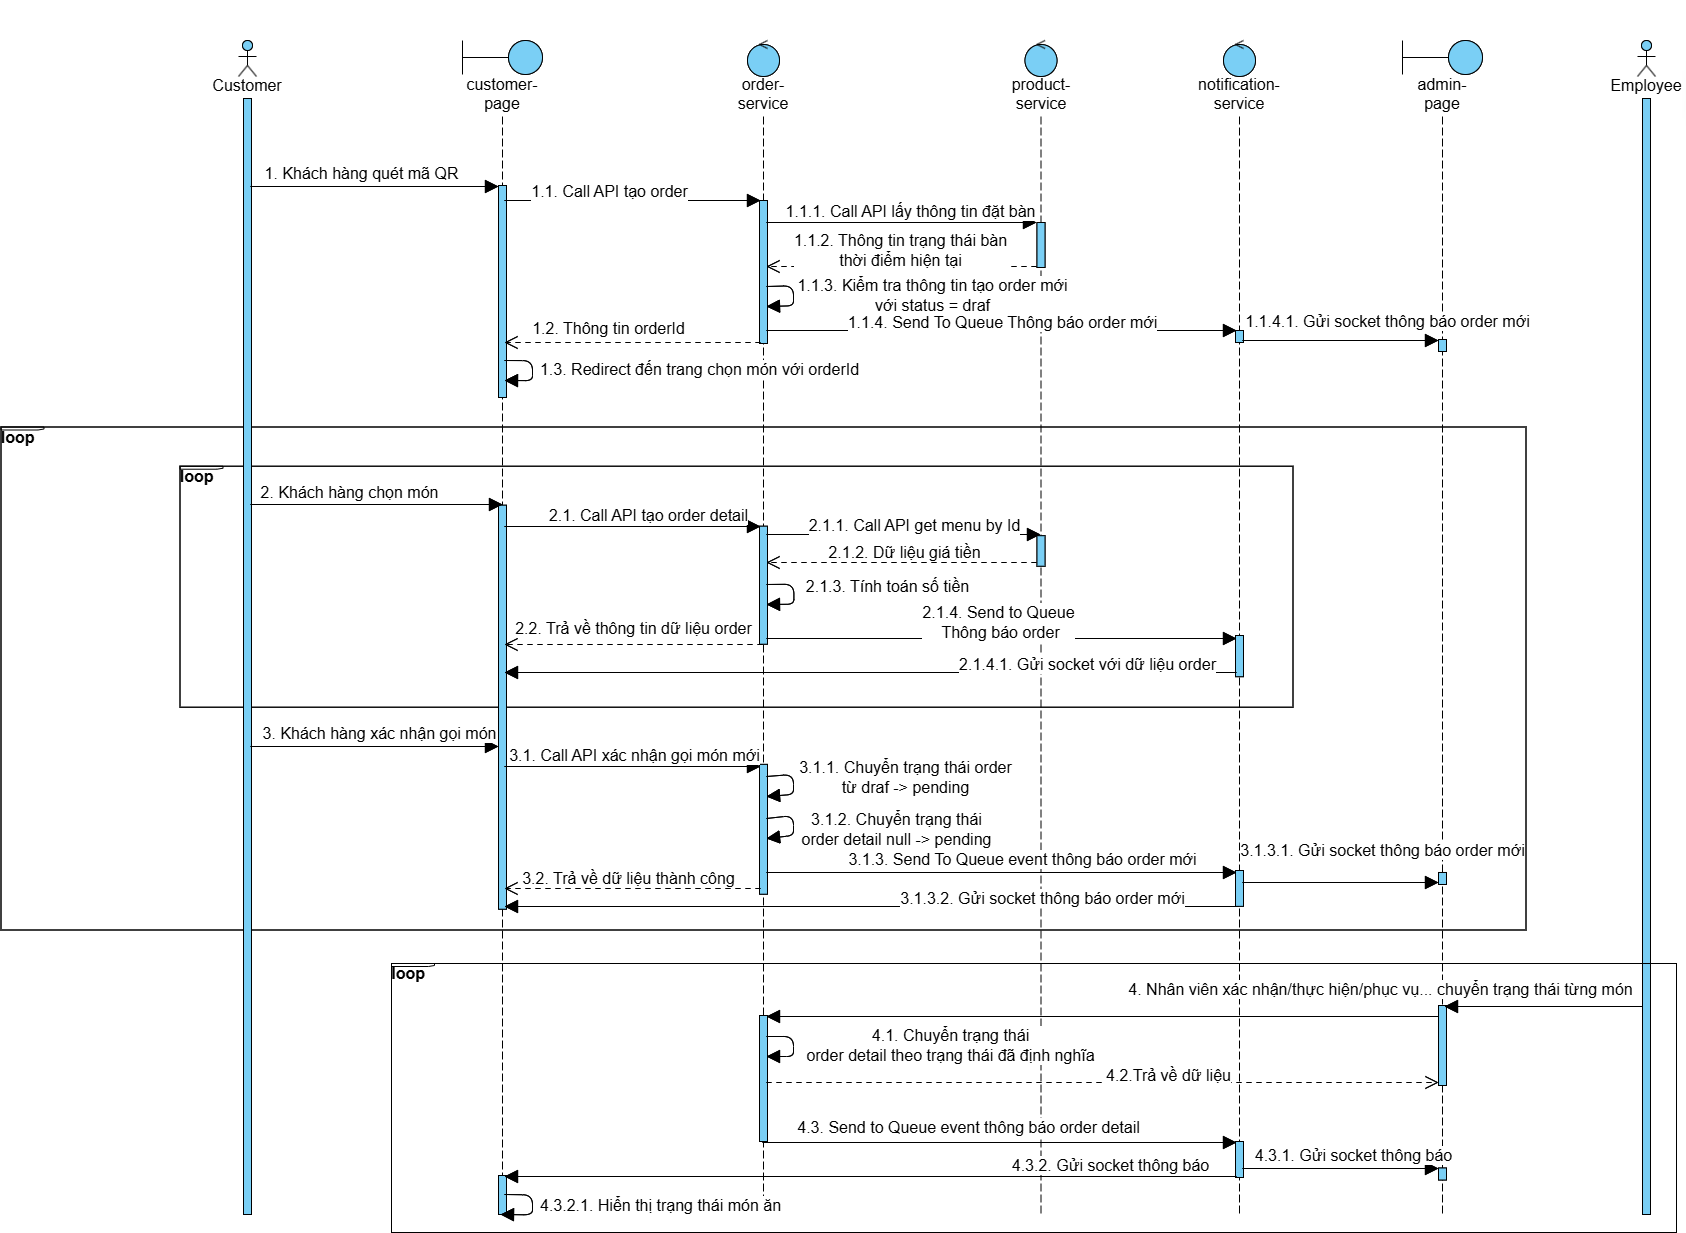
\includegraphics[width=1.1\textwidth]{images/hChip/main-flow/order.png}
	\caption{Sơ đồ tuần tự mô tả luồng nghiệp vụ đặt món thông qua quét mã QR}
	\label{fig:order-sequence-flow}
\end{figure}

Sau khi người dùng thực hiện quét mã QR, hệ thống sẽ thực hiện xác nhận tạo order mới cho số bàn đang ngồi với trạng thái là \tcode{draf}.
Khách hàng sẽ được chuyển hướng đến trang chọn món sau khi nhận lại \tcode{orderId}, ở đấy khách hàng sẽ chọn các món ăn từ thực đơn của quán.
Sau khi người dùng hoàn thành quá trình chọn đồ ăn cũng như xác nhận danh sách các món ăn cho đơn hàng, nhân viên, phục vụ, đầu bếp, v.v. sẽ chuyển trạng thái từng món cụ thể dựa theo tình trạng hiện tại của món ăn như \textit{đang chuẩn bị}, \textit{dã xong}, \textit{đã phục vụ}, v.v.
Toàn bộ luồng nghiệp vụ sẽ lặp lại cho đến khi người dùng chọn tính năng thanh toán và hoàn thành bữa ăn.
% \begin{table}[h]
%     \centering
%     \caption{Kết quả thời gian chuẩn bị môi trường trên ba mô-đun thực nghiệm}
%     \label{tab:time_undef}
% \begin{tabular}{|l|l|l|l|ll|}
% \hline
% \multicolumn{1}{|c|}{\multirow{2}{*}{\textbf{Module}}} & \multicolumn{1}{c|}{\multirow{2}{*}{\textbf{File}}} & \multicolumn{1}{c|}{\multirow{2}{*}{\textbf{Undef}}} & \multirow{2}{*}{\textbf{Compilable}} & \multicolumn{2}{c|}{\textbf{Linkable}} \\ \cline{5-6} 
% \multicolumn{1}{|c|}{}                                 & \multicolumn{1}{c|}{}                               & \multicolumn{1}{c|}{}                                &                                      & \multicolumn{1}{l|}{Manual}  & Propose \\ \hline
% collision (Box2d)                                      & 53                                                  & 5                                                    & 0:02:39                              & \multicolumn{1}{l|}{0:08:23} & 0:00:04 \\ \hline
% FPT1                                     & 45                                                  & 263                                                  & 1:04:22                              & \multicolumn{1}{l|}{0:14:48} & 0:00:28 \\ \hline
% FPT2                                          & 126                                                 & 333                                                  & 2:05:56                              & \multicolumn{1}{l|}{1:31:01} & 0:02:24 \\ \hline
% \end{tabular}
% \end{table}      